\documentclass{standalone}
\usepackage{tikz, amsmath, subfigure}
\usetikzlibrary{calc}
\usetikzlibrary{decorations.pathreplacing,calligraphy}
\usetikzlibrary{snakes}
\usepackage{xcolor}

\begin{document}

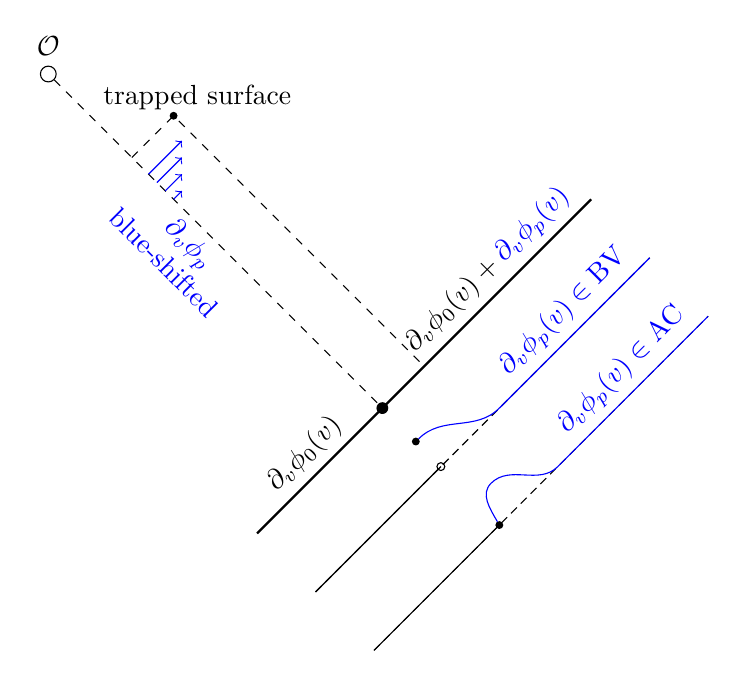
\begin{tikzpicture}[scale = 1.5]
\node[circle, label= above:{$\mathcal{O}$}, draw, inner sep =0, minimum size = .2cm] (n1) at (0,0) {};
\draw[dashed] (n1) -- (-45:4);
\draw[thick] ($(-45:4) + (-135:1.5)$ ) -- ($(-45:4) + (45:2.5)$ );
\node[circle,fill,inner sep =0, minimum size = .15cm] (n2) at ($(-45:4)$) {};

\node[label = {[rotate=45,yshift=-1mm]above:$\partial_v \phi_0(v)$ }] at ($(-45:4) + (-135:.8)$ ) {};
\node[label = {[rotate=45,yshift=-1mm]above:$\partial_v \phi_0(v) + \color{blue}\partial_v \phi_p(v)$ }] at ($(-45:4) + (45:1.4)$ ) {};

\coordinate (c1) at ($(-45:4) + (-135:1.5) + (-45:.7)$ );
\coordinate (c2) at ($(-45:4) + (45:2.5) + (-45:.7)$ );
\coordinate (m1) at ($(-45:4) + (-45:.7)$ );

\draw[densely dashed] (c1) -- (c2);
\node[circle, draw, inner sep =0, minimum size = .1cm]  at (m1) {};
\draw[] (c1)--(m1);

\node[circle, draw,fill, inner sep = .03cm] (n10) at ($(m1) + (135:.3) $ ) { };

\draw[blue] (n10) to[out=45, in = -135] ($(m1) + (45:.7)$) ;
\draw[blue] ($(m1) + (45:.7)$) to  ($(m1) + (45:.7) + (45:1.8)$) ;


\node[label={[rotate=45, yshift=-1mm]above:{ \color{blue}$\partial_v \phi_p(v) \in \text{BV}$}   }] at ($(c2) + (-135:.9) $){};



\coordinate (c3) at ($(-45:4) + (-135:1.5) + (-45:1.4)$ );
\coordinate (c4) at ($(-45:4) + (45:2.5) + (-45:1.4)$ );
\coordinate (m2) at ($(-45:4) + (-45:1.4)$ );

\draw[densely dashed] (c3) -- (c4);
\node[label={[rotate=45, yshift=-1mm]above:{ \color{blue}$\partial_v \phi_p(v) \in \text{AC}$}   }] at ($(c4) + (-135:.9) $){};
\draw[] (c3)--(m2);

\node[circle, draw,fill, inner sep = .03cm] (n11) at ($(m2)  $ ) { };
\draw[blue] (n11) to[out=120, in = -135] ($(m2) + (45:.2) + (135:.3)$) ;
\draw[blue] ($(m2) + (45:.2) + (135:.3)$) to[out=45, in = -135] ($(m2) + (45:.7) $)  ;
\draw[blue] ($(m2) + (45:.7) $) to ($(m2) + (45:.7) + (45:1.8)$)  ;

\coordinate (d1) at (-45:1);
\coordinate (d2) at ($(-45:1) + (45:.5)$);
\coordinate (d3) at (-45:4);
\coordinate (d4) at ($(-45:4) + (45:.5)$);

\draw[dashed] (d1) -- (d2) --(d4) -- (d3);
\node[circle, draw, fill,inner sep = .03cm, label={[xshift=3mm, yshift=-1mm]above:{  {trapped  surface}  }}  ] at (d2) {};

\coordinate (d5) at (-45:1.2);
\coordinate (d6) at (-45:1.3);
\coordinate (d7) at (-45:1.4);
\coordinate (d8) at (-45:1.5);
\draw[blue,->] (d5) to ($(d5)+(45:.4)$);
\draw[blue,->] (d6) to ($(d6)+(45:.3)$);
\draw[blue,->] (d7) to ($(d7)+(45:.2)$);
\draw[blue,->] (d8) to ($(d8)+(45:.1)$);

\node[label={[align=center, rotate=-45,xshift=6mm,yshift=1mm]below:{  \color{blue}$\partial_v \phi_p$ \\  \color{blue}blue-shifted }}] at (d7) {};


\end{tikzpicture}
\end{document}